\documentclass[xcolor=table]{beamer}
\usepackage{beamerthemesplit}
\usepackage{wrapfig}
\usetheme{SPbGU}
\usepackage{pdfpages}
\usepackage{amsmath}
\usepackage{cmap}
\usepackage[T2A]{fontenc}
\usepackage[utf8]{inputenc}
\usepackage[english]{babel}
\usepackage{indentfirst}
\usepackage{amsmath}
\usepackage{tikz}
\usepackage{multirow}
\usepackage[noend]{algpseudocode}
\usepackage{algorithm}
\usepackage{algorithmicx}
\usepackage{fancyvrb}
\usetikzlibrary{shapes,arrows}
%usepackage{fancyvrb}
%\usepackage{minted}
%\usepackage{verbments}

\newtheorem{mytheorem}{Theorem}
\renewcommand{\thealgorithm}{}


\beamertemplatenavigationsymbolsempty

\title[CFPQ]{Context-Free Path Querying by Matrix Multiplication}
%\subtitle[YaccConstructor]{Parsing techniques for graph analysis}
% То, что в квадратных скобках, отображается в левом нижнем углу.
\institute[JetBrains Research]{
JetBrains Research, Programming Languages and Tools Lab  \\
Saint Petersburg University
}

% То, что в квадратных скобках, отображается в левом нижнем углу.
\author[Kate Verbitskaia]{Rustam Azimov, Semyon Grigorev \\ presents Kate Verbitskaia}

\date{June 10, 2018}

\definecolor{orange}{RGB}{179,36,31}

\begin{document}
{
\begin{frame}[fragile]
  \begin{tabular}{p{3.5cm} p{5.5cm} p{1cm}}
   \begin{center}
      
\includegraphics[height=1.5cm]{pictures/jetbrainsResearch.pdf}
    \end{center}
    &
    \begin{center}
      % 
\includegraphics[height=1.5cm]{pictures/SLELogo.png}
    \end{center}
    &
    \begin{center}
      
\includegraphics[height=1.5cm]{pictures/SPbGU_Logo.png}
    \end{center}
  \end{tabular}
  \titlepage
\end{frame}
}

\begin{frame}[fragile]
  \transwipe[direction=90]
  \frametitle{Context-Free Path Querying}
\begin{minipage}[m]{0.45\linewidth}
\raisebox{-0.5\totalheight}{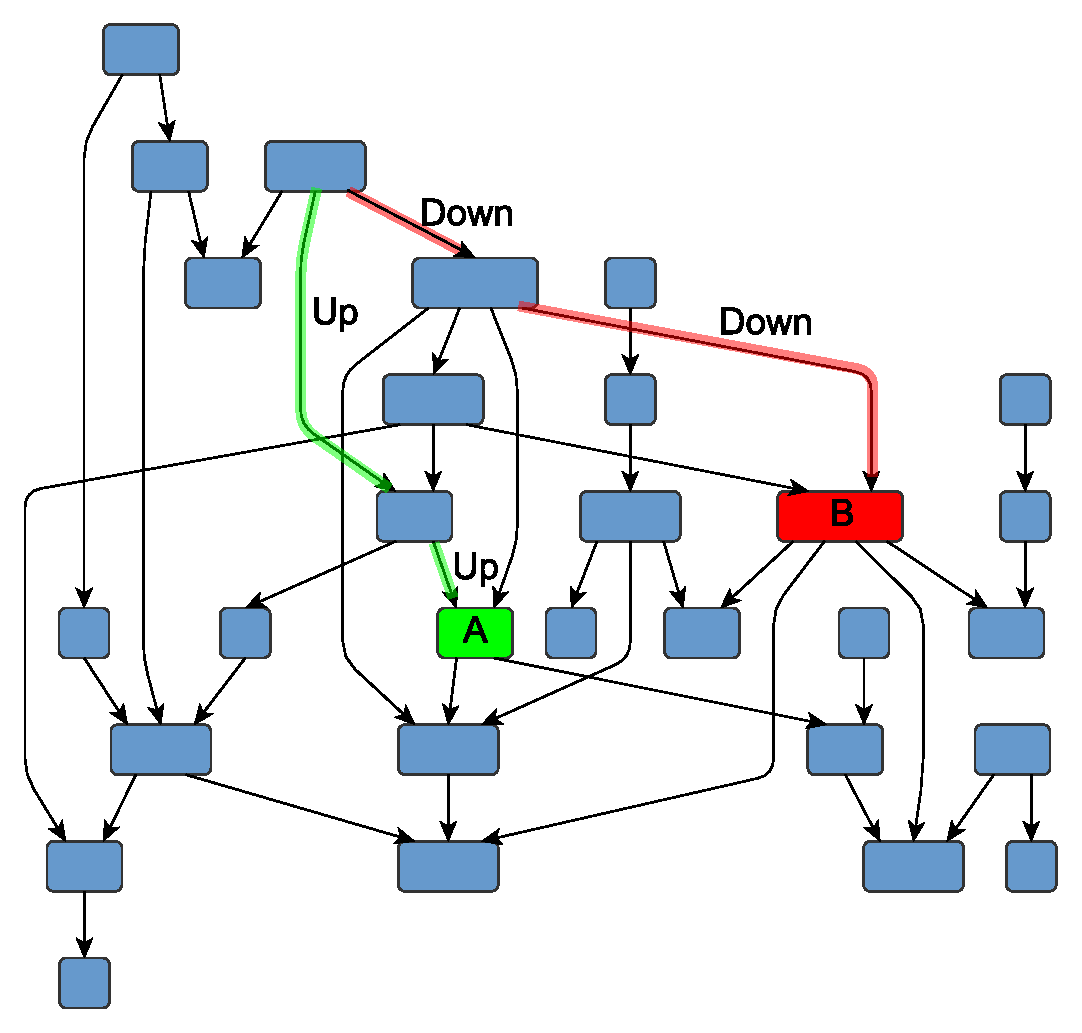
\includegraphics[width=\textwidth]{pictures/hierarchical.pdf}}
\end{minipage}\hfill
\begin{minipage}[m]{0.5\linewidth}
Navigation through a graph
\begin{itemize}
      \item Are nodes A and B on the same level of hierarchy?
      \item Is there a path of form $\textbf{Up}^n \, \textbf{Down}^n$?
      \item Find all paths of form $\textbf{Up}^n \, \textbf{Down}^n$ which start from the~node A
\end{itemize}

\end{minipage}

\end{frame}

\begin{frame}[fragile]
  \transwipe[direction=90]
  \frametitle{Context-Free Path Querying: Relational Query Semantics}
  \begin{itemize}
    \item $\mathbb{G} = (\Sigma, N, P)$ --- context-free grammar in normal form
    \begin{itemize}
      \item $A \rightarrow B C$, where $A, B, C \in N$
      \item $A \rightarrow x$, where $A \in N, x \in \Sigma$
      \item $L(\mathbb{G},A) = \{ \omega \mid A \rightarrow^* \omega \}$
    \end{itemize}
    \item $G = (V,E,L)$ --- directed graph
      \begin{itemize}
        \item $v \xrightarrow{l} u \in E$
        \item $L \subseteq \Sigma$
      \end{itemize}
    %\item $p = v_0 \xrightarrow{l_0} v_1 \xrightarrow{l_1} \cdots \xrightarrow{l_{n-2}} v_{n-1} \xrightarrow{l_{n-1}} v_n$ --- path in $G$
    \item $\omega(\pi) = \omega(v_0 \xrightarrow{l_0} v_1 \xrightarrow{l_1} \cdots \xrightarrow{l_{n-2}} v_{n-1} \xrightarrow{l_{n-1}} v_n) = l_0 l_1 \cdots l_{n-1}$
    \item $R_A = \{ (n, m) \mid \exists n \pi m$, such that $\omega(\pi) \in L(\mathbb{G},A)\}$
  \end{itemize}
\end{frame}

\begin{frame}[fragile]
  \transwipe[direction=90]
  \frametitle{Regular Language Constraints}
  \begin{itemize}
   \item Widely spread
    \begin{itemize}
      \item Graph databases query languages (SPARQL, Cypher, PGQL)
      \item Network analysis
    \end{itemize}
    \item Still in active development
    \begin{itemize}
      \item OpenCypher: \url{https://goo.gl/5h5a8P}
      \item Scalability, huge graphs processing
      \item Derivatives for graph querying: \emph{Maurizio Nole and Carlo Sartiani.} Regular path queries on massive graphs. 2016
    \end{itemize}
  \end{itemize}
\end{frame}


\begin{frame}[fragile]
  \transwipe[direction=90]
  \frametitle{Context-Free Language Constraints}
  \begin{itemize}
  \item Graph databases and semantic networks (Context-Free Path Querying, CFPQ)
    \begin{itemize}
        \item \emph{Sevon P., Eronen L.} ``Subgraph queries by context-free grammars.'' 2008
        \item \emph{Hellings J.} ``Conjunctive context-free path queries.'' 2014
        \item \emph{Zhang X. et al.} ``Context-free path queries on RDF graphs.'' 2016
    \end{itemize}
    \item Static code analysis (Language Reachability Framework)
    \begin{itemize}
        \item \emph{Thomas Reps et al.} ``Precise interprocedural dataflow analysis via graph reachability.'' 1995
        \item \emph{Qirun Zhang et al.}  ``Efficient subcubic alias analysis for C.'' 2014
        \item \emph{Dacong Yan et al.} ``Demand-driven context-sensitive alias analysis for Java.'' 2011
        \item \emph{Jakob Rehof and Manuel Fahndrich.} ``Type-base flow analysis: from polymorphic subtyping to CFL-reachability.'' 2001
    \end{itemize}
  \end{itemize}
\end{frame}


%\begin{frame}
%  \transwipe[direction=90]
%  \frametitle{Context-free language constraints}
%
%\begin{itemize}
%\item Interprocedural static nullability analysis\footnote{\emph{Kai Wang et. al.} Graspan: a single-machine disk-based graph system for interprocedural
%static analyses of large-scale systems code. 2017}
%
%\begin{itemize}
%   \item ``We have identified a total of 1127 unnecessary NULL tests in Linux, 149 in PostgreSQL,
%   32 in httpd.''
%   \item ``Our analyses reported 108 new NULL pointer dereference bugs in Linux, among which 23 are false positives''
%   \item ``For PostgreSQL and httpd, we detected 33 and 14 new NULL pointer bugs; our manual
%   validation did not find any false positives among them.''
%\end{itemize}
%
%\end{itemize}
%
%\end{frame}

%\begin{frame}
%  \transwipe[direction=90]
%  \frametitle{Existing Approaches}
%  \begin{itemize}
%    \item Do not use the power of advanced parsing techniques
%    \begin{itemize}
%       \item Are mostly based on CYK \\ (Zhang, et al. ``Context-Free Path Queries on RDF Graphs.''; \\ Hellings. ``Conjunctive Context-Free Path Queries.'')
%       \item Do not provide useful structural representation of result
%     \end{itemize}
%    \item Impose restrictions on input
%    \begin{itemize}
%       \item Do not process input graphs with cycles \\ (Sevon, Eronen. ``Subgraph Queries by Context-Free Grammars.'')
%       \item Are restricted to certain grammar classes
%     \end{itemize}
%  \end{itemize}
%\end{frame}

\begin{frame}
  \transwipe[direction=90]
  \frametitle{Open Problems}
  \begin{itemize}
    \item Development of efficient algorithms
    \item Effective utilization of GPGPU and parallel programming
    \item Lifting up the limitations on the input graph and the query language
  \end{itemize}
\end{frame}

\begin{frame}
  \transwipe[direction=90]
  \frametitle{The algorithm}

\begin{algorithm}[H]
\begin{algorithmic}[1]
\caption{Context-free recognizer for graphs}
\label{alg:graphParse}
\Function{contextFreePathQuerying}{D, G}

    \State{$n \gets$ the number of nodes in $D$}
    \State{$E \gets$ the directed edge-relation from $D$}
    \State{$P \gets$ the set of production rules in $G$}
    \State{$T \gets$ the matrix $n \times n$ in which each element is $\varnothing$}
    \ForAll{$(i,x,j) \in E$}
    \Comment{Matrix initialization}
        \State{$T_{i,j} \gets T_{i,j} \cup \{A~|~(A \rightarrow x) \in P \}$}
    \EndFor
    \While{matrix $T$ is changing}

        \State{$T \gets T \cup (T \times T)$}
        \Comment{Transitive closure $T^{cf}$ calculation}
    \EndWhile
\State \Return $T$
\EndFunction
\end{algorithmic}
\end{algorithm}

\end{frame}


\begin{frame}[fragile]
  \transwipe[direction=90]
  \frametitle{Derivation Step}

  \begin{tabular}{p{4cm} | p{6cm} }
      $$ A \rightarrow x $$

   \begin{center}
      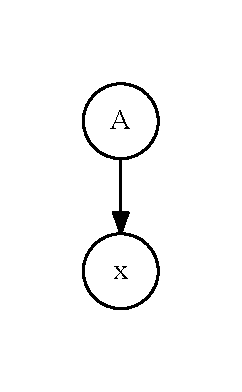
\includegraphics[height=3.5cm]{pictures/tree1.pdf}
    \end{center}

    &
      $$ A \rightarrow B C $$

    \begin{center}
      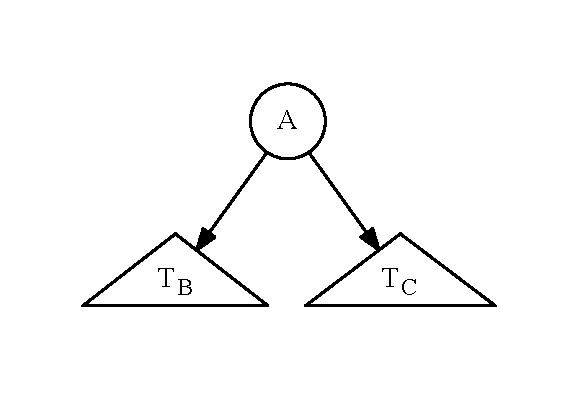
\includegraphics[height=3.5cm]{pictures/tree2.pdf}
    \end{center}
  \end{tabular}

\end{frame}

\begin{frame}
  \transwipe[direction=90]
  \frametitle{Matrix Multiplication}
  \begin{itemize}
    \item Subset multiplication, $N_1, N_2 \subseteq N$
    \begin{itemize}
      \item $N_1 \cdot N_2 = \{A~|~\exists B \in N_1, \exists C \in N_2 \text{ such that }(A \rightarrow B C) \in P\}$
    \end{itemize}
    \item Subset addition: set-theoretic union.
  \end{itemize}

  \begin{itemize}
    \item Matrix multiplication
    \begin{itemize}
      \item Matrix of size $|V| \times |V|$
      \item Subsets of $N$ are elements
      \item $c_{i,j} = \bigcup^{n}_{k=1}{a_{i,k} \cdot b_{k,j}}$
    \end{itemize}
  \end{itemize}
\end{frame}

\begin{frame}
  \transwipe[direction=90]
  \frametitle{Transitive Closure}
  \begin{itemize}
    \item $a^{cf} = a^{(1)} \cup a^{(2)} \cup \cdots$
    \item $a^{(1)} = a$
    \item $a^{(i)} = a^{(i-1)} \cup (a^{(i-1)} \times a^{(i-1)}), ~i \ge 2$
  \end{itemize}
\end{frame}

\begin{frame}
  \transwipe[direction=90]
  \frametitle{The algorithm}

\begin{algorithm}[H]
\begin{algorithmic}[1]
\caption{Context-free recognizer for graphs}
\label{alg:graphParse}
\Function{contextFreePathQuerying}{D, G}

    \State{$n \gets$ the number of nodes in $D$}
    \State{$E \gets$ the directed edge-relation from $D$}
    \State{$P \gets$ the set of production rules in $G$}
    \State{$T \gets$ the matrix $n \times n$ in which each element is $\varnothing$}
    \ForAll{$(i,x,j) \in E$}
    \Comment{Matrix initialization}
        \State{$T_{i,j} \gets T_{i,j} \cup \{A~|~(A \rightarrow x) \in P \}$}
    \EndFor
    \While{matrix $T$ is changing}

        \State{$T \gets T \cup (T \times T)$}
        \Comment{Transitive closure $T^{cf}$ calculation}
    \EndWhile
\State \Return $T$
\EndFunction
\end{algorithmic}
\end{algorithm}

\end{frame}

\begin{frame}
  \transwipe[direction=90]
  \frametitle{Algorithm Correctness}
\begin{mytheorem}
 Let $D = (V,E)$ be a graph and let $G =(N,\Sigma,P)$ be a grammar.

 Then for any $i, j$ and for any non-terminal $A \in N$, $A \in a^{cf}_{i,j}$ iff $(i,j) \in R_A$.
\end{mytheorem}


\begin{mytheorem}
 Let $D = (V,E)$ be a graph and let $G =(N,\Sigma,P)$ be a grammar.

 The Algorithm~\ref{alg:graphParse} terminates in a finite number of steps.
\end{mytheorem}
\end{frame}

\begin{frame}
  \transwipe[direction=90]
  \frametitle{Algorithm Complexity}
\begin{mytheorem}
 Let $D = (V,E)$ be a graph and let $G =(N,\Sigma,P)$ be a grammar. The~Algorithm~\ref{alg:graphParse} calculates the transitive closure $T^{cf}$ in $O(|V|^2|N|^3(BMM(|V|) + BMU(|V|)))$.
\end{mytheorem}

\begin{itemize}
  \item $BMM(n)$ --- number of elementary operations executed by the
algorithm of multiplying two $n \times n$ Boolean matrices.
  \item $BMU(n)$ --- number of elementary operations, executed by the matrix union
operation of two $n \times n$ Boolean matrices
\end{itemize}

\end{frame}


\begin{frame}[fragile]
  \transwipe[direction=90]
  \frametitle{Algorithm Complexity: the Worst Case}



Input graph: two cycles connected via a shared node

\begin{itemize}
	\item first cycle has $2^k + 1$ edges labeled $a$
	\item second cycle has $2^k$ edges labeled $b$
\end{itemize}


\begin{tabular}{p{3cm} p{7cm} }
\begin{figure}[h]
	\[
	\begin{array}{ccl}
	S & \rightarrow & \text{\emph{a}} \ S \ \text{\emph{b}} \\
	  & |           & \text{\emph{a}} \ \text{\emph{b}} \\
	\end{array}
	\]

\end{figure}

&

\begin{center}
  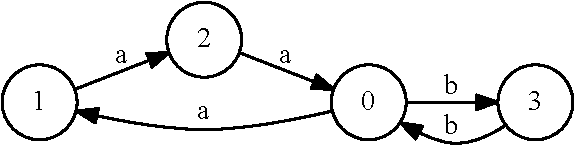
\includegraphics[height=2cm]{pictures/example_graph.pdf}
\end{center}
  \end{tabular}
\end{frame}

\begin{frame}
  \transwipe[direction=90]
  \frametitle{The Worst Case: Step by Step}
\begin{tabular}{p{3cm} p{7cm} }
\begin{figure}[h]
   \[
\begin{array}{ccl}
    S & \rightarrow & A \ B \\
      & | & A \ S_1 \\
    S_1 & \rightarrow & S \ B \\
    A & \rightarrow & \text{\emph{a}} \\
    B & \rightarrow & \text{\emph{b}} \\
\end{array}
\]
\label{ProductionRulesExampleQueryCNF}
\end{figure}

&

\begin{figure}[h]
\[
T_0 = \begin{pmatrix}
    \varnothing & \{A\}       & \varnothing & \{B\}       \\
    \varnothing & \varnothing & \{A\}       & \varnothing \\
    \{A\}       & \varnothing & \varnothing & \varnothing \\
    \{B\}       & \varnothing & \varnothing & \varnothing \\
\end{pmatrix}
\]

\end{figure}
 \end{tabular}

\begin{center}
  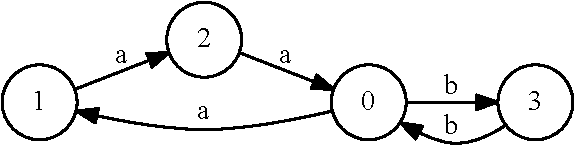
\includegraphics[height=2cm]{pictures/example_graph.pdf}
\end{center}

\end{frame}

\begin{frame}[noframenumbering]
  \transwipe[direction=90]
  \frametitle{The Worst Case: Step by Step}
\begin{figure}[h]
\[
T_0 \times T_0 = \begin{pmatrix}
	\varnothing & \varnothing & \varnothing & \varnothing \\
	\varnothing & \varnothing & \varnothing & \varnothing \\
	\varnothing & \varnothing & \varnothing & \{S\}       \\
	\varnothing & \varnothing & \varnothing & \varnothing \\
\end{pmatrix}
\]

\[
T_1 = T_0 \cup (T_0 \times T_0) = \begin{pmatrix}
	\varnothing & \{A\}       & \varnothing & \{B\}       \\
	\varnothing & \varnothing & \{A\}       & \varnothing \\
	\{A\}       & \varnothing & \varnothing & \{\pmb{S}\}       \\
	\{B\}       & \varnothing & \varnothing & \varnothing \\
\end{pmatrix}
\]
\label{ExampleQueryFirstIteration}
\end{figure}
\end{frame}

\begin{frame}[noframenumbering]
  \transwipe[direction=90]
  \frametitle{The Worst Case: Step by Step}
\begin{figure}[h]
\[
T_2 = \begin{pmatrix}
    \varnothing & \{A\}       & \varnothing & \{B\}       \\
    \varnothing & \varnothing & \{A\}       & \varnothing \\
    \{A, \pmb{S_1}\}  & \varnothing & \varnothing & \{S\}       \\
    \{B\}       & \varnothing & \varnothing & \varnothing \\
\end{pmatrix}
\]
\label{ExampleQueryFirstIteration}
\end{figure}
\end{frame}

\begin{frame}[noframenumbering]
  \transwipe[direction=90]
  \frametitle{The Worst Case: Step by Step}
\begin{figure}[h]
\[
T_3 = \begin{pmatrix}
\varnothing & \{A\}       & \varnothing & \{B\}       \\
\{\pmb{S}\}       & \varnothing & \{A\}       & \varnothing \\
\{A, S_1\}  & \varnothing & \varnothing & \{S\}       \\
\{B\}       & \varnothing & \varnothing & \varnothing \\
\end{pmatrix}
\]
\label{ExampleQueryFirstIteration}
\end{figure}
\end{frame}

\begin{frame}[noframenumbering]
  \transwipe[direction=90]
  \frametitle{The Worst Case: Step by Step}
\begin{figure}[h]
\[
T_4 = \begin{pmatrix}
\varnothing & \{A\}       & \varnothing & \{B\}       \\
\{S\}       & \varnothing & \{A\}       & \{\pmb{S_1}\}     \\
\{A, S_1\}  & \varnothing & \varnothing & \{S\}       \\
\{B\}       & \varnothing & \varnothing & \varnothing \\
\end{pmatrix}
\]
\label{ExampleQueryFirstIteration}
\end{figure}
\end{frame}

\begin{frame}[noframenumbering]
  \transwipe[direction=90]
  \frametitle{The Worst Case: Step by Step}
\begin{figure}[h]
\[
T_5 = \begin{pmatrix}
\varnothing & \{A\}       & \varnothing & \{B, \pmb{S}\}    \\
\{S\}       & \varnothing & \{A\}       & \{S_1\}     \\
\{A, S_1\}  & \varnothing & \varnothing & \{S\}       \\
\{B\}       & \varnothing & \varnothing & \varnothing \\
\end{pmatrix}
\]
\label{ExampleQueryFirstIteration}
\end{figure}
\end{frame}

\begin{frame}[noframenumbering]
  \transwipe[direction=90]
  \frametitle{The Worst Case: Step by Step}
\begin{figure}[h]
\[
T_6 = \begin{pmatrix}
\{\pmb{S_1}\}     & \{A\}       & \varnothing & \{B, S\}    \\
\{S\}       & \varnothing & \{A\}       & \{S_1\}     \\
\{A, S_1\}  & \varnothing & \varnothing & \{S\}       \\
\{B\}       & \varnothing & \varnothing & \varnothing \\
\end{pmatrix}
\]
\label{ExampleQueryFirstIteration}
\end{figure}
\end{frame}

\begin{frame}[noframenumbering]
  \transwipe[direction=90]
  \frametitle{The Worst Case: Step by Step}
\begin{figure}[h]
\[
T_7 = \begin{pmatrix}
\{S_1\}     & \{A\}       & \varnothing & \{B, S\}    \\
\{S\}       & \varnothing & \{A\}       & \{S_1\}     \\
\{A, S_1, \pmb{S}\}  & \varnothing & \varnothing & \{S\}    \\
\{B\}       & \varnothing & \varnothing & \varnothing \\
\end{pmatrix}
\]
\label{ExampleQueryFirstIteration}
\end{figure}
\end{frame}

\begin{frame}[noframenumbering]
  \transwipe[direction=90]
  \frametitle{The Worst Case: Step by Step}
\begin{figure}[h]
\[
T_8 = \begin{pmatrix}
\{S_1\}     & \{A\}       & \varnothing & \{B, S\}    \\
\{S\}       & \varnothing & \{A\}       & \{S_1\}     \\
\{A, S_1, S\}  & \varnothing & \varnothing & \{S, \pmb{S_1}\} \\
\{B\}       & \varnothing & \varnothing & \varnothing \\
\end{pmatrix}
\]
\label{ExampleQueryFirstIteration}
\end{figure}
\end{frame}

\begin{frame}[noframenumbering]
  \transwipe[direction=90]
  \frametitle{The Worst Case: Step by Step}
\begin{figure}[h]
\[
T_9 = \begin{pmatrix}
\{S_1\}     & \{A\}       & \varnothing & \{B, S\}    \\
\{S\}       & \varnothing & \{A\}       & \{S_1, \pmb{S}\}     \\
\{A, S_1, S\}  & \varnothing & \varnothing & \{S, S_1\} \\
\{B\}       & \varnothing & \varnothing & \varnothing \\
\end{pmatrix}
\]
\label{ExampleQueryFirstIteration}
\end{figure}
\end{frame}

\begin{frame}[noframenumbering]
  \transwipe[direction=90]
  \frametitle{The Worst Case: Step by Step}
\begin{figure}[h]
\[
T_{10} = \begin{pmatrix}
\{S_1\}     & \{A\}       & \varnothing & \{B, S\}    \\
\{S, \pmb{S_1}\}       & \varnothing & \{A\}       & \{S_1, S\}     \\
\{A, S_1, S\}  & \varnothing & \varnothing & \{S, S_1\} \\
\{B\}       & \varnothing & \varnothing & \varnothing \\
\end{pmatrix}
\]
\label{ExampleQueryFirstIteration}
\end{figure}
\end{frame}

\begin{frame}[noframenumbering]
  \transwipe[direction=90]
  \frametitle{The Worst Case: Step by Step}

\begin{figure}[h]
\[
T_{11} = \begin{pmatrix}
\{S_1, \pmb{S}\}     & \{A\}       & \varnothing & \{B, S\}    \\
\{S, S_1\}       & \varnothing & \{A\}       & \{S_1, S\}     \\
\{A, S_1, S\}  & \varnothing & \varnothing & \{S, S_1\} \\
\{B\}       & \varnothing & \varnothing & \varnothing \\
\end{pmatrix}
\]
\label{ExampleQueryFirstIteration}
\end{figure}
\end{frame}

\begin{frame}[noframenumbering]
  \transwipe[direction=90]
  \frametitle{The Worst Case: Step by Step}

\begin{figure}[h]
\[
T_{12} = \begin{pmatrix}
\{S_1, S\}     & \{A\}       & \varnothing & \{B, S, \pmb{S_1}\}    \\
\{S, S_1\}       & \varnothing & \{A\}       & \{S_1, S\}     \\
\{A, S_1, S\}  & \varnothing & \varnothing & \{S, S_1\} \\
\{B\}       & \varnothing & \varnothing & \varnothing \\
\end{pmatrix}
\]
\label{ExampleQueryFirstIteration}
\end{figure}
\end{frame}

\begin{frame}[noframenumbering]
  \transwipe[direction=90]
  \frametitle{The Worst Case: Step by Step}

\begin{figure}[h]
\[
T_{13} = \begin{pmatrix}
\{S_1, S\}     & \{A\}       & \varnothing & \{B, S, S_1\}    \\
\{S, S_1\}       & \varnothing & \{A\}       & \{S_1, S\}     \\
\{A, S_1, S\}  & \varnothing & \varnothing & \{S, S_1\} \\
\{B\}       & \varnothing & \varnothing & \varnothing \\
\end{pmatrix}
\]
\label{ExampleQueryFirstIteration}
\end{figure}
\end{frame}

\begin{frame}
  \transwipe[direction=90]
  \frametitle{Evaluation}

\begin{itemize}
    \item dGPU (dense GPU): row-major matrix representation and a GPU for matrix operation calculation.
    \item sCPU (sparse CPU): CSR format for sparse matrix representation and a CPU for matrix operation calculation.
    \item sGPU (sparse GPU): CSR format for sparse matrix representation and a GPU for matrix operation calculation.
\end{itemize}


\end{frame}


\begin{frame}
  \transwipe[direction=90]
  \frametitle{Evaluation: Same Generation Queries}
Query 1 retrieves the concepts on the same layer

\begin{figure}[h]
   \[
\begin{array}{ccl}
   S & \rightarrow & \text{\emph{subClassOf}}^{-1} \ S \ \text{\emph{subClassOf}} \\
     & |           & \text{\emph{type}}^{-1} \ S \ \text{\emph{type}} \\
     & |           & \text{\emph{subClassOf}}^{-1} \ \text{\emph{subClassOf}} \\
     & |           & \text{\emph{type}}^{-1} \ \text{\emph{type}} \\
\end{array}
\]

\end{figure}

Query 2 retrieves concepts on the adjacent layers

\begin{figure}[h]
   \[
\begin{array}{ccl}
   S & \rightarrow & B \ \text{\emph{subClassOf}} \\
     & |           & \text{\emph{subClassOf}} \\
   B & \rightarrow & \text{\emph{subClassOf}}^{-1} \ B \ \text{\emph{subClassOf}} \\
     & |           & \text{\emph{subClassOf}}^{-1} \ \text{\emph{subClassOf}} \\
\end{array}
\]
\end{figure}

\end{frame}

\begin{frame}
  \transwipe[direction=90]
  \frametitle{Evaluation: Query 1}
\begin{tabular}{  c | c | c | c | c | c | c | c }
%\hline
Ontology & V & E & \#results & GLL & dGPU & sCPU & sGPU\\
%\hline
\hline
skos        & 144 & 323 & 810 & 10 & 56 & 14 & 12\\
generations & 129 & 351 & 2164 & 19 & 62 & 20 & 13\\
travel      & 131 & 397 & 2499 & 24 & 69 & 22 & 30\\
univ-bench  & 179 & 413 & 2540 & 25 & 81 & 25 & 15\\
atom-prim   & 291 & 685 & 15454 & 255 & 190 & 92 & 22\\ %atom-primitive
biomedical  & 341 & 711 & 15156 & 261 & 266 & 113 & 20\\ % biomedical-measure-primitive
foaf        & 256 & 815 & 4118 & 39 & 154 & 48 & 9\\
people-pets & 337 & 834 & 9472 & 89 & 392 & 142 & 32\\
funding     & 778 & 1480 & 17634 & 212 & 1410 & 447 & 36\\
wine        & 733 & 2450 & 66572 & 819 & 2047 & 797 & 54\\
pizza       & 671 & 2604 & 56195 & 697 & 1104 & 430 & 24\\
$g_{1}$     & 6224 & 11840 & 141072 & 1926 & --- & 26957 & 82\\
$g_{2}$     & 5864 & 19600 & 532576 & 6246 & --- & 46809 & 185\\
$g_{3}$     & 5368 & 20832 & 449560 & 7014 & --- & 24967 & 127\\
%\hline
\end{tabular}

\begin{center} time is measured in ms \end{center}
    \end{frame}

\begin{frame}
  \transwipe[direction=90]
  \frametitle{Evaluation: Query 2}
\begin{tabular}{ c | c | c | c | c | c | c | c }
%\hline
Ontology & V & E & \#results & GLL & dGPU & sCPU & sGPU\\
%\hline
\hline
skos        & 144 & 323 & 1 & 1 & 10 & 2 & 1\\
generations & 129 & 351 & 0 & 1 & 9 & 2 & 0\\
travel      & 131 & 397 & 63 & 1 & 31 & 7 & 10\\
univ-bench  & 179 & 413 & 81 & 11 & 55 & 15 & 9\\
atom-prim   & 291 & 685 & 122 & 66 & 36 & 9 & 2\\
biomedical  & 341 & 711 & 2871 & 45 & 276 & 91 & 24\\  % biomedical-measure-primitive
foaf        & 256 & 815 & 10 & 2 & 53 & 14 & 3\\
people-pets & 337 & 834 & 37 & 3 & 144 & 38 & 6\\
funding     & 778 & 1480 & 1158 & 23 & 1246 & 344 & 27\\
wine        & 733 & 2450 & 133 & 8 & 722 & 179 & 6\\
pizza       & 671 & 2604 & 1262 & 29 & 943 & 258 & 23\\
$g_{1}$     & 6224 & 11840 & 9264 & 167 & --- & 21115 & 38\\
$g_{2}$     & 5864 & 19600 & 1064 & 46 & --- & 10874 & 21\\
$g_{3}$     & 5368 & 20832 & 10096 & 393 & --- & 15736 & 40\\
%\hline
\end{tabular}

\begin{center} time is measured in ms \end{center}
\end{frame}


\begin{frame}
  \transwipe[direction=90]
  \frametitle{Summary}
\begin{itemize}
\item Algorithm for context-free path querying
\item Works on any input graph
\item Supports any context-free constraints
\item Is independent of matrix representation
\item Can utilize GPGPU easily and efficiently
\end{itemize}
\end{frame}

\begin{frame}
\transwipe[direction=90]
\frametitle{Contact Information}
\begin{itemize}
  \item Semyon Grigorev: \href{mailto:s.v.grigoriev@spbu.ru}{s.v.grigoriev@spbu.ru}
  \item Rustam Azimov: \href{mailto:st013567@student.spbu.ru}{st013567@student.spbu.ru}
\end{itemize}
\begin{itemize}
  \item YaccConstructor: \href{https://github.com/YaccConstructor}{https://github.com/YaccConstructor}
\end{itemize}
\end{frame}
\end{document}
